\documentclass{beamer}

\synctex=1

\mode<presentation>
{
  \usetheme{Warsaw}
  \setbeamercovered{invisible}
}

\setbeamertemplate{navigation symbols}{}
%\setbeamertemplate{footline}[frame number]{}

\graphicspath{ {./images/} }

\usepackage[british]{babel}
\usepackage{times}
\usepackage[latin1]{inputenc}
\usepackage[T1]{fontenc}
\usepackage{lmodern}
\usepackage{amsmath,amsthm,amssymb}
\usepackage{hyperref}
\usepackage{nccfoots}
\usepackage{subfigure}

\renewcommand\thempfootnote{*}

\renewcommand{\t}{$\mathrm{t}$}
\newcommand{\BHV}{$\mathrm{BHV}$}
\newcommand{\NP}{$\mathrm{NP}$}
\newcommand{\MCMC}{$\mathrm{MCMC}$}
\newcommand{\SPR}{$\mathrm{SPR}$}

\newcommand{\dts}{\mathrm{2DtT}}
\newcommand{\nni}{\mathrm{NNI}}
\newcommand{\rnni}{\mathrm{rNNI}}
\newcommand{\rnniu}{\mathrm{rNNIu}}
\newcommand{\mdts}{\mathrm{DtT}}
\newcommand{\mdtsu}{\mathrm{DtTu}}
\newcommand{\MH}{\mathrm{MH}}
\newcommand{\ric}{\operatorname{ric}}
\newcommand{\rt}{\mathrm{rt}}
\newcommand{\tp}{\mathrm{tp}}
\newcommand{\W}{\mathcal{W}}
\newcommand{\M}{\mathcal{M}}
\newcommand{\dom}{\mathrm{dom}}

\renewcommand{\O}{\mathcal{O}}


\newtheorem{oobservation}{Trivial observation}
\newtheorem{answer}{Answer}

\theoremstyle{example}
\newtheorem{question}{Question}

\title[\url{http://gavruskin.github.io/talks/AWC_2015.pdf}]{AWC Anual Meeting:\\
Convergence and curvature of phylogenetic Markov chains}
\author[These slides:]{Alex Gavryushkin\\
(joint work with Chris Whidden and Erick Matsen)}
\titlegraphic{
\includegraphics[height=2cm]{UniAuckland}}

\date{21st October 2015}

\begin{document}

\begin{frame}[plain]
\titlepage
\end{frame}

\begin{frame}{Motivation}
\begin{question}
Why all Bayesian phylogeny inference software is (sometimes / so) slow?
\end{question}

\pause

\begin{question}
Specifically: Why does it take (sometimes / so) much time to converge?
\end{question}

\pause

\begin{question}
Even more specifically: Why no reliable convergence criterion is know?
\end{question}

\begin{answer}
\pause
I don't know
\pause
geometry well.
\end{answer}
\end{frame}

\begin{frame}{Discrete time-trees}
\begin{definition}[Ranked tree topology]
\begin{figure}
\centering
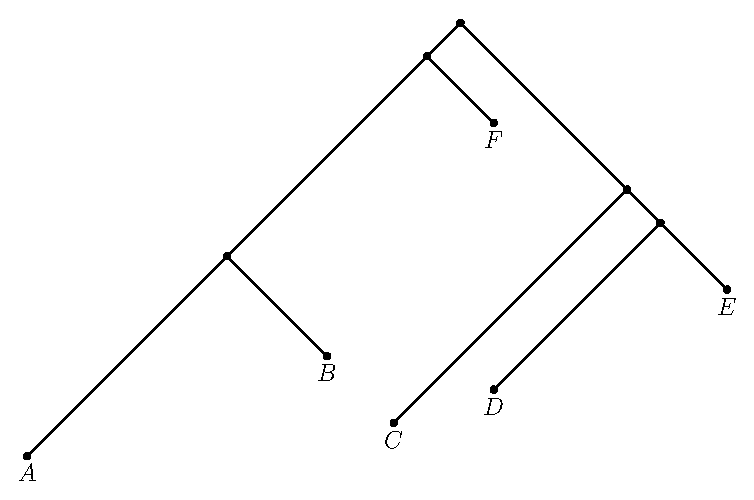
\includegraphics[width = \framewidth]{ranked_tree.eps}
\end{figure}
\end{definition}
\end{frame}

\begin{frame}{Discrete time-trees}
\begin{definition}[Ranked tree topology]
\begin{figure}
\centering
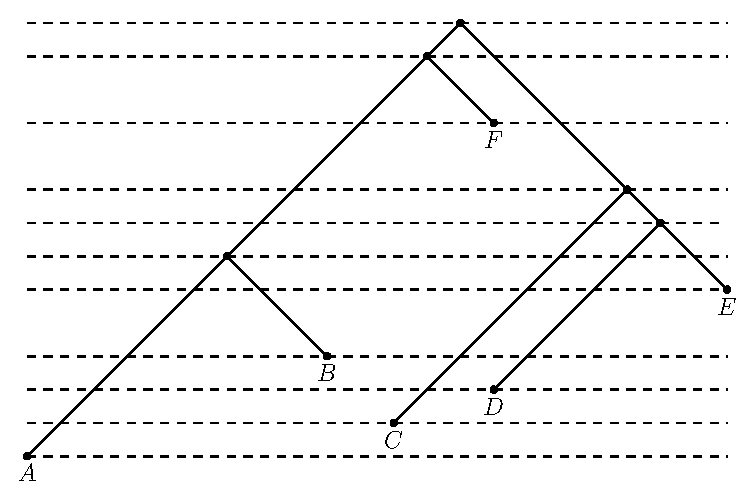
\includegraphics[width = \framewidth]{ranked_tree_dashed.eps}
\end{figure}
\end{definition}
\end{frame}

\begin{frame}{Discrete time-trees}
\begin{definition}[Discrete time-tree]
\begin{figure}
\centering
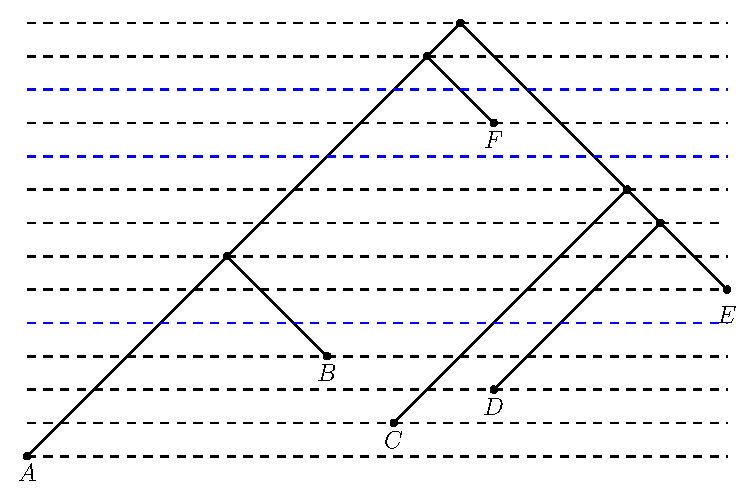
\includegraphics[width = \framewidth]{ranked_tree_dashed_time.eps}
\end{figure}
\end{definition}
\end{frame}

\begin{frame}{Discrete time-tree space}
\centering
{\small\color{blue} ~~~~~~~~~~ Trees at distance 3}
\vskip-8mm
\begin{figure}
\centering
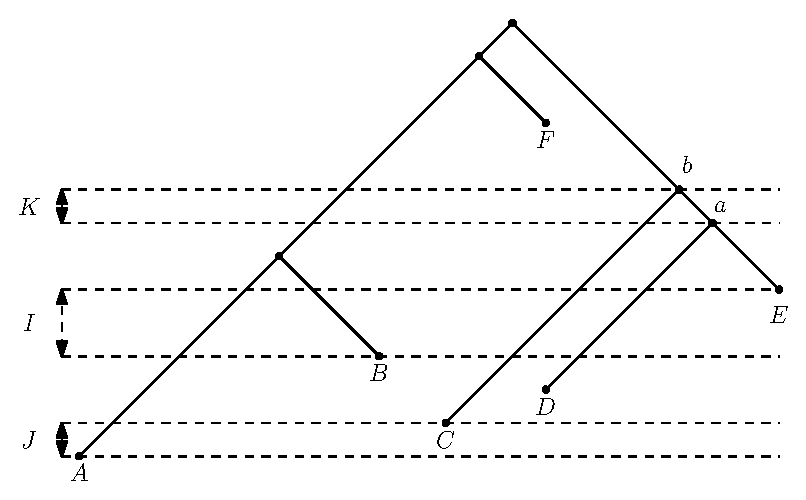
\includegraphics[width=.53\framewidth]{dts_neighbours_left.eps}
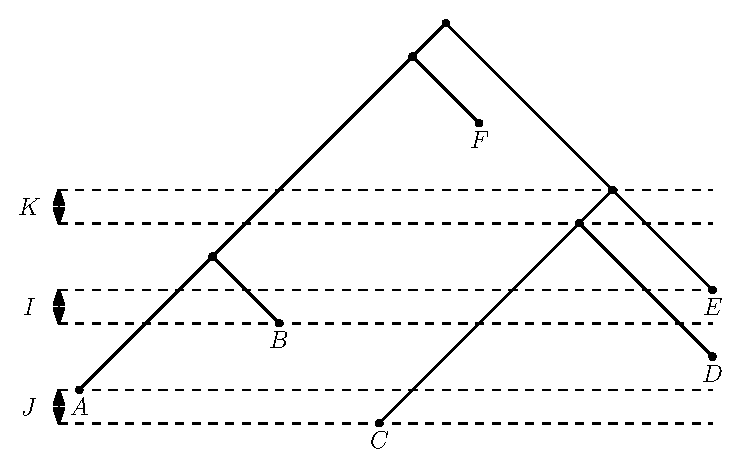
\includegraphics[width=.53\framewidth]{dts_neighbours_right.eps}
\end{figure}

\pause

\begin{figure}
\centering
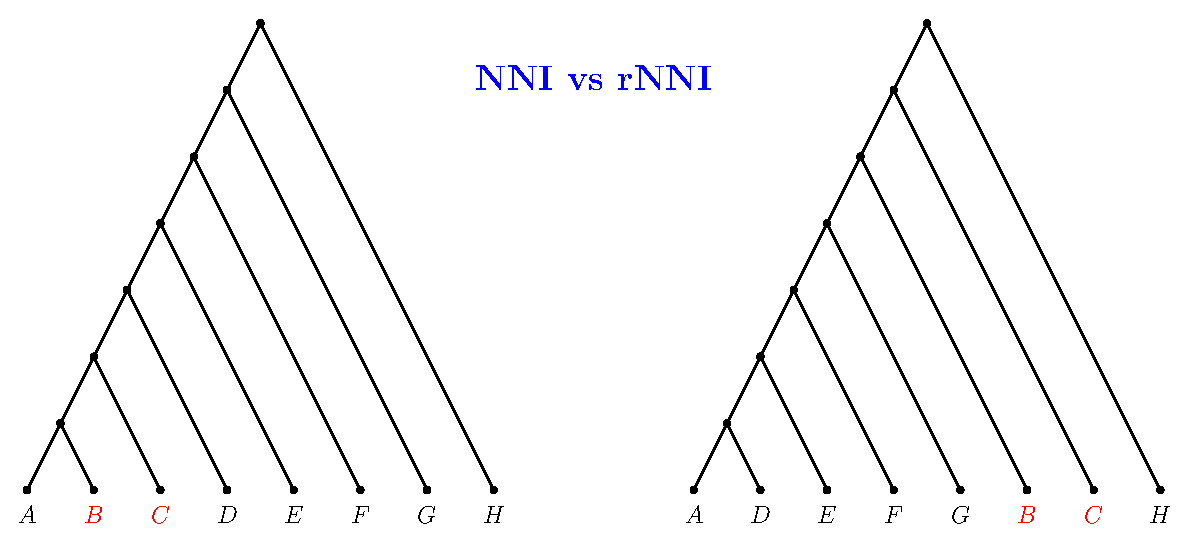
\includegraphics[width=.8\framewidth]{dts_nni.eps}
\end{figure}

\end{frame}

\begin{frame}{Ricci-Ollivier curvature}
\begin{definition}[Ollivier~{[2009]}]
Let $({\cal T},d)$ be a metric (tree) space with a random walk
\vskip-3mm
\[
m = (m_T)_{T\in{\cal T}}.
\]
Let $T,R \in {\cal T}$ be two distinct points (trees).
The Ricci-Ollivier curvature of $({\cal T},d,m)$ along $\overrightarrow{TR}$ is
\vskip-3mm
\[
\kappa_m(T,R) = 1 - \frac{W(m_T ,m_R)}{d(T,R)},
\]
where $W(\cdot\,,\cdot)$ is the earth mover's distance.
\end{definition}
\end{frame}

\begin{frame}{In a nutshell}
\begin{block}{Negative VS positive}
\centering
$\kappa_m(T, R) \leq 0 \iff W(m_T, m_R) \geq d(T, R)$
\end{block}

\pause

\begin{block}{Take-home message}
Negative curvature is bad.
\end{block}
\end{frame}

\begin{frame}{Curvature of Markov chains on graphs}

\begin{theorem}[Ollivier~{[2009]}]
If $({\cal T}, d)$ is a geodesic space then curvature is a local property.
\end{theorem}

\begin{definition}
Let $({\cal T}, d)$ be a graph with a Markov chain $m$.Then the {\em curvature of the Markov chain} $m$ on the graph $\cal T$ is the greatest number $\chi_m$ such that
\vskip-5mm
\[
\chi_m \leq \kappa_m(T,R) \mbox{ for adjacent $T$ and $R$}.
\]
\end{definition}

\begin{oobservation}
Under a distance-one random walk, the following is true for any finite metric $d$ and any pair of points $T, R$:
\vskip-3mm
\[
\dfrac{-2}{d(T, R)} \leq \kappa(T, R) \leq \dfrac{2}{d(T, R)}.
\]
\end{oobservation}
\end{frame}

\begin{frame}{Random walks}
For now, we consider three simplest random walks on various phylogenetic tree spaces.

\begin{itemize}
\item Metropolis-Hastings random walk: Choose a tree from the one neighbourhood and accept it with probability $\min(1, \dfrac{|N_1(T_{old})|}{|N_1(T_{new})|})$.
\item Uniform random walk.
\item Uniform $p$-lazy random walk, where $p$ is the laziness probability.
\end{itemize}
\end{frame}

\begin{frame}{Lower bounds}
\begin{theorem}[G, Whidden, Matsen {[2015]}]
Let $T$ and $R$ be adjacent trees.
Then both the asymptotic curvature of the space with $p$-lazy uniform random walk and the curvature of the space with uniform random walk are at least 
\begin{align*}
& \kappa(T,R) \geq \frac{-n^2 + 2n}{3.5n^2 - 15n + 16} \geq -2/5	&& \mbox{in $\mathrm rSPR$ space,}\\
& \kappa(T,R) \geq -\dfrac{4}{n-1}							&& \mbox{in $\mdts$ space,}\\
& \kappa(T,R) \geq -\dfrac{4}{n-2}							&& \mbox{in $\nni$ space,}\\
& \kappa(T,R) \geq -\dfrac{8}{n-1}							&& \mbox{in $\rnni$ space.}
\end{align*}

The bounds are tight.
\end{theorem}
\end{frame}

\begin{frame}{Upper bounds}
\begin{theorem}[G, Whidden, and Matsen {[2015]}]
Let $T$ and $R$ be adjacent trees.
Then the curvature of the following spaces with uniform random walk satisfy
\begin{align*}
& \kappa(T,R) \leq \frac{6n-17}{3n^2-13n+14}	&& \mbox{in $\mathrm{rSPR}$ space,}\\
& \kappa(T,R) \leq \dfrac{1}{2(n-1)}			&& \mbox{in $\mdts$ space,}\\
& \kappa(T,R) \leq \dfrac{1}{2(n-2)}			&& \mbox{in $\nni$ space, and}\\
& \kappa(T,R) \leq \dfrac{1}{n-1}				&& \mbox{in $\rnni$ space.}
\end{align*}
The bounds are tight.
\end{theorem}
\end{frame}

\begin{frame}{Life is good, at infinity}
\begin{theorem}[G, Whidden, and Matsen {[2015]}]
Let $\{T_n \mid n \in \mathbb N\}$ and $\{S_n \mid n \in \mathbb N\}$ be two sequences of phylogenetic trees such that $d(T_n,R_n) = 1$ for all $n$.
Then $$\lim_{n \rightarrow \infty} \kappa_n(T_n,S_n) = 0$$ for the uniform random walk on the SPR
graph\footnote{For the SPR graph, we have to bound the size of the subtree which is getting moved.},
the $\nni$ graph, the $\rnni$-graph, and the $\mdts$-graph.
\end{theorem}
\end{frame}

\begin{frame}{Whidden and Matsen [2015]}
\begin{figure}
\hspace*{\stretch{1}}
\subfigure[6 taxa]{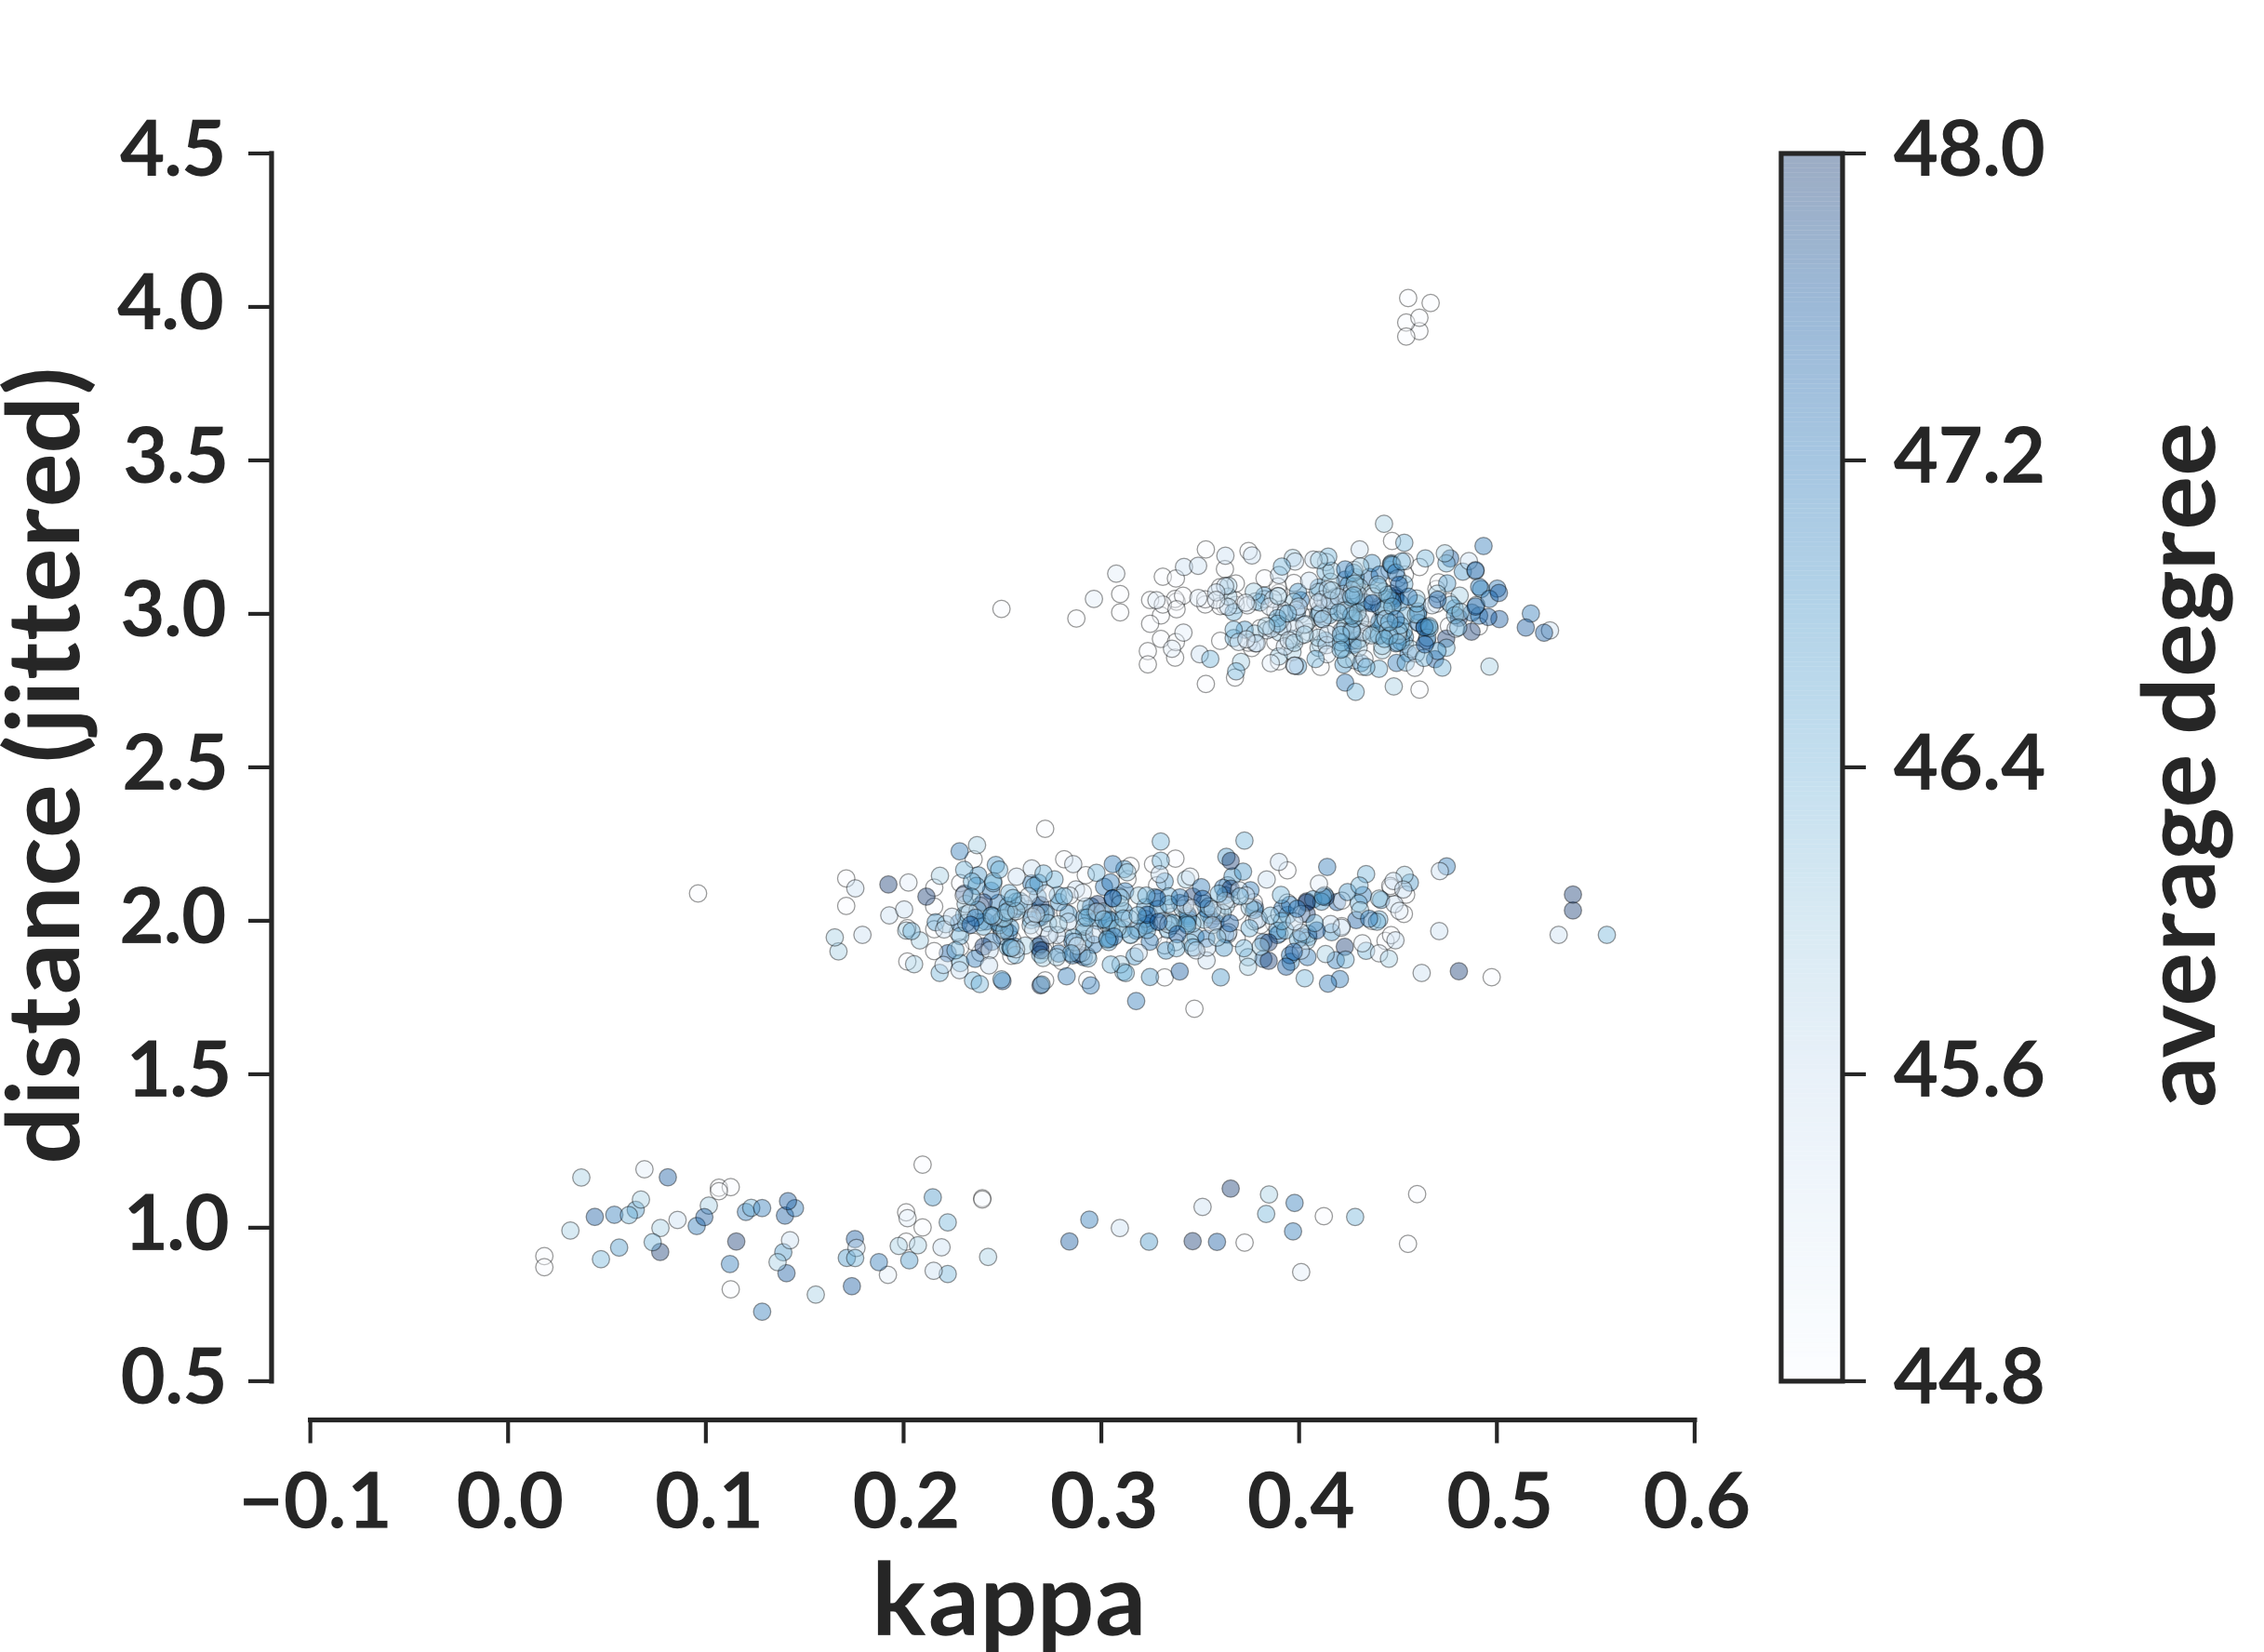
\includegraphics[width=.48\framewidth]{rspr-upmh-scatter6}}
\hspace*{\stretch{2}}
\subfigure[7 taxa]{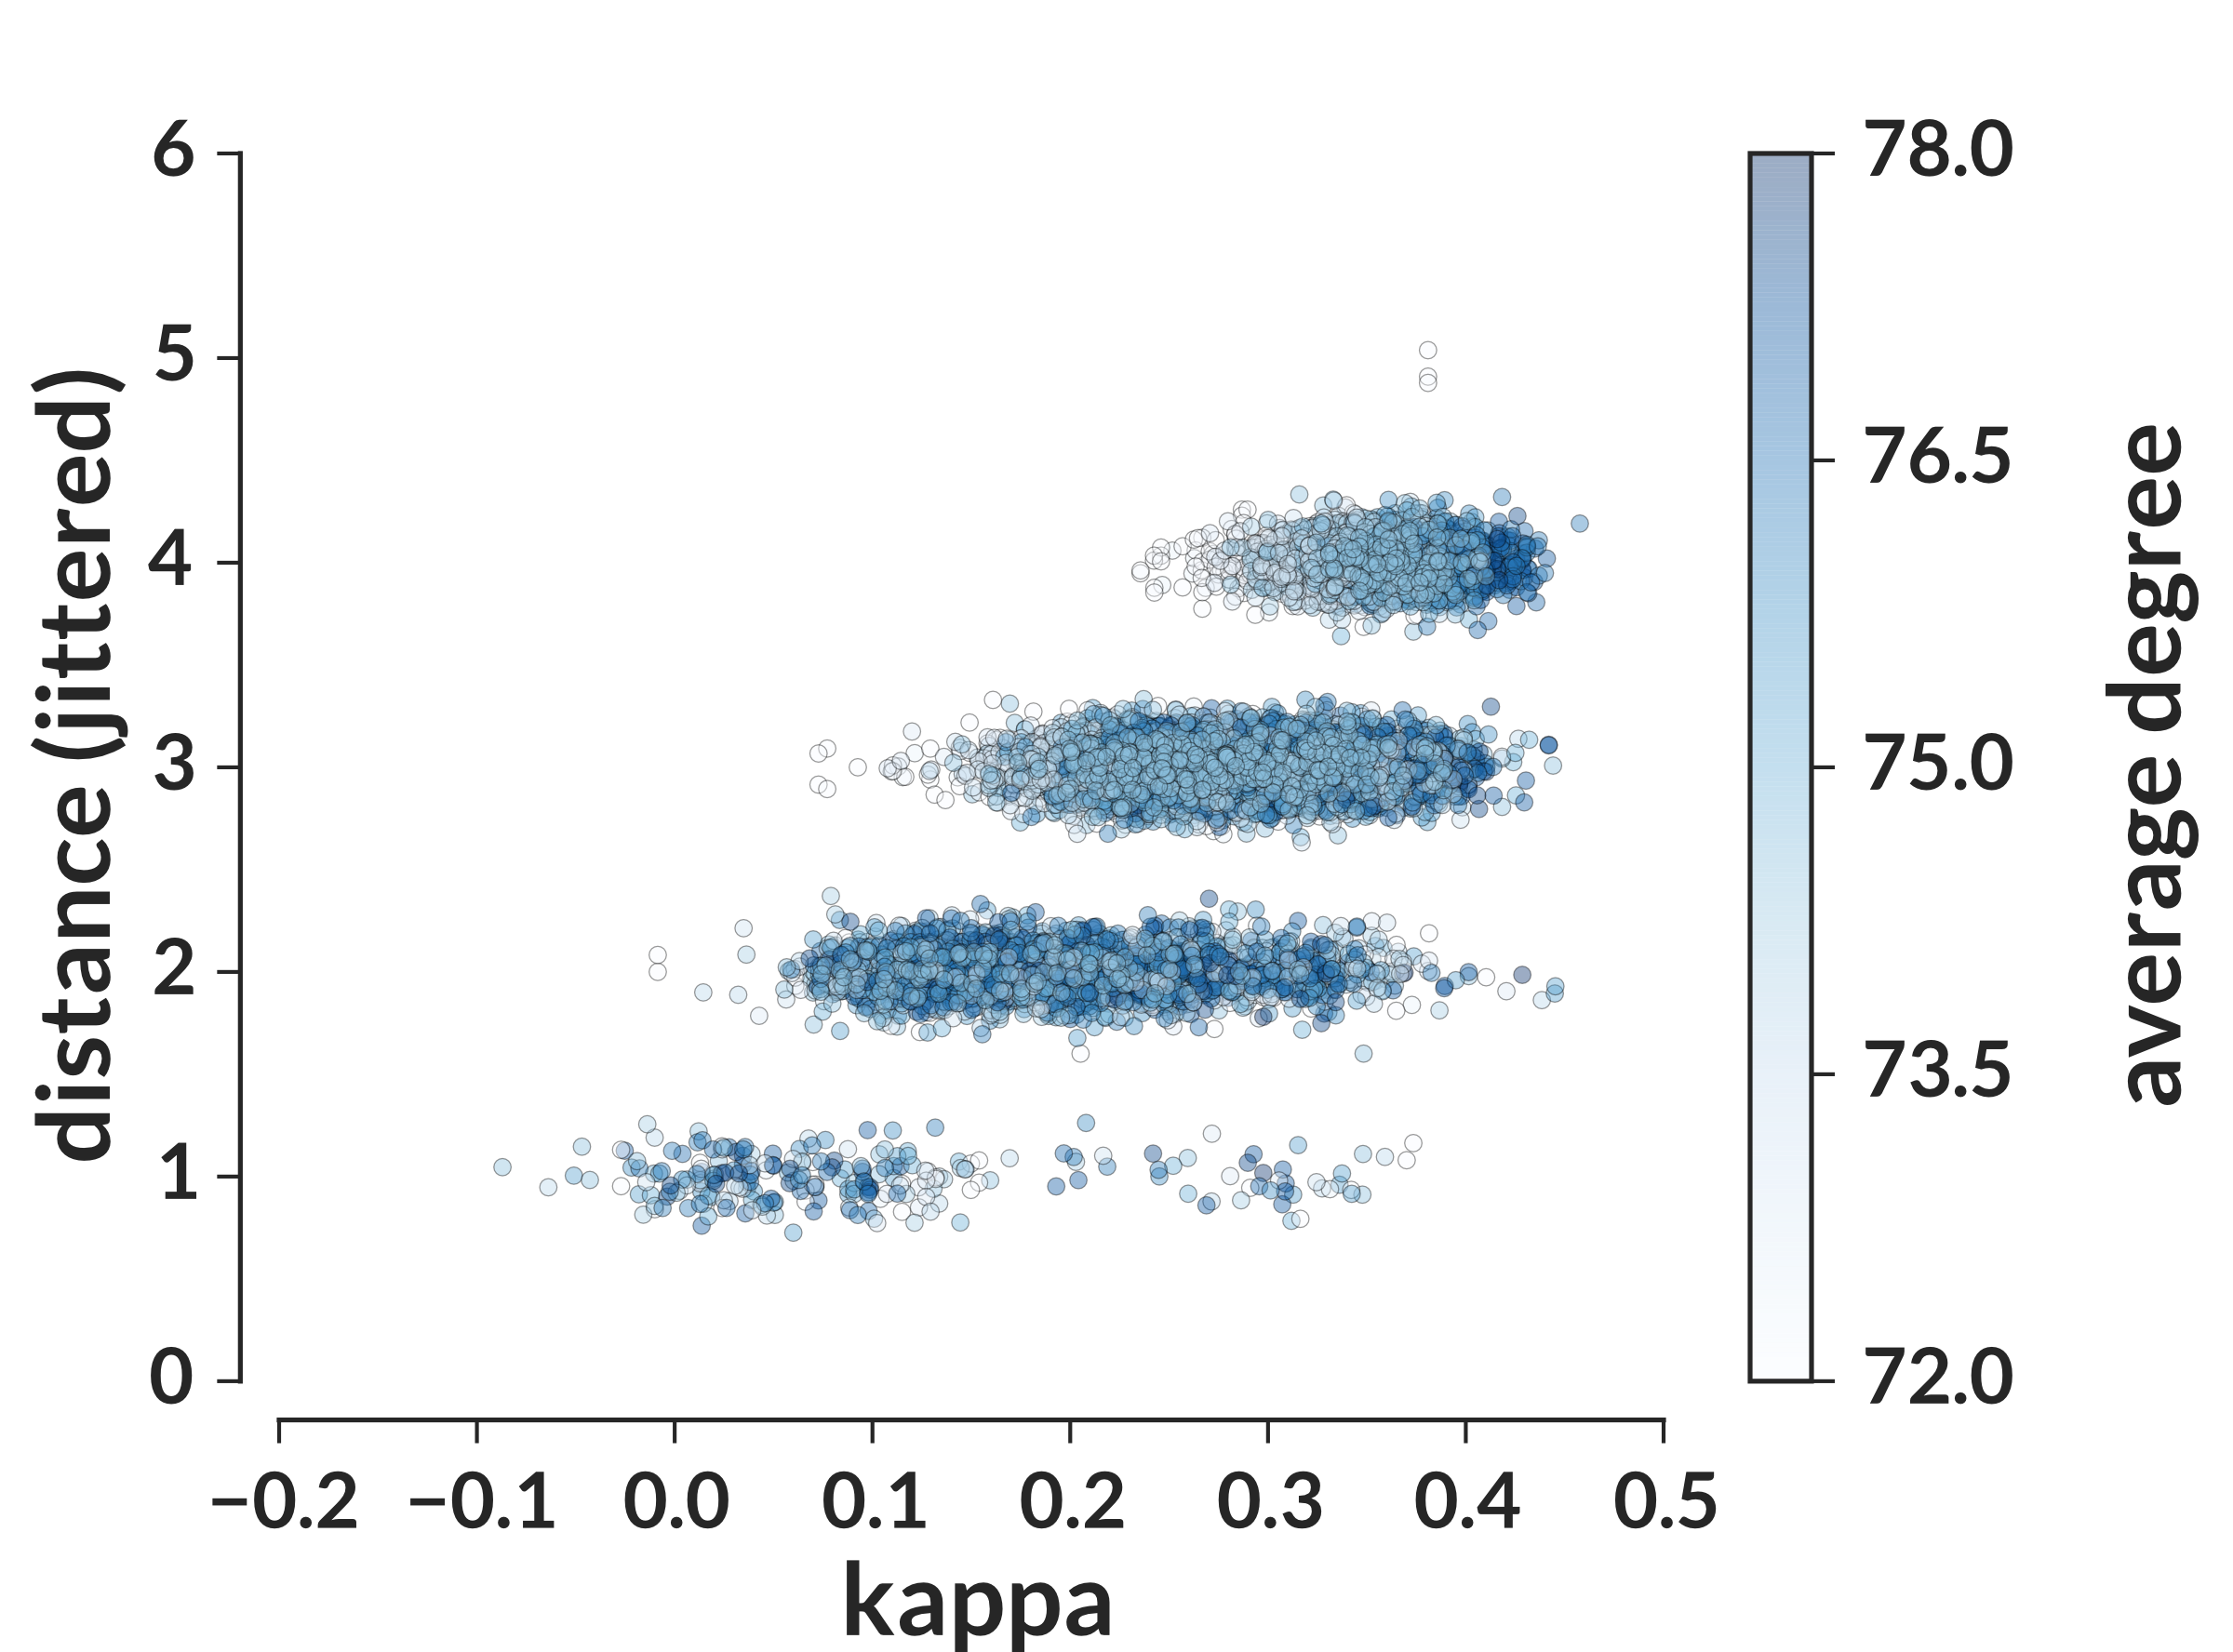
\includegraphics[width=.48\framewidth]{rspr-upmh-scatter7}}
\hspace*{\stretch{1}}
    \caption{\small Scatter plot of $\kappa(\mathrm{MH}; T_1,T_2)$ values versus $d_{SPR}(T_1,T_2)$ for the rSPR graph. Colour displays the average degree of $T_1$ and $T_2$. Distance values randomly perturbed (``jittered'') a small amount to avoid superimposed points.}
\end{figure}
\end{frame}

\begin{frame}{Take-home message}
\begin{block}{}
\[
1.001^{10000} = 21916.68\ldots
\]
\[
\mbox{BUT}
\]
\[
0.999^{10000} = 0.000045\ldots
\]
\end{block}

\pause

\begin{block}{}
\begin{itemize}
\item The curvature of basic random walks is normally positive.
\item Although the spaces flatten out when the number of taxa $n$ grows, there always are negatively curved pieces.
\item Importantly, the number of those pieces grows with $n$.
\end{itemize}
\end{block}
\end{frame}

\begin{frame}{\href{http://alex.gavruskin.com/pictures/}{\Large{Thank
you for your attention!}}}
\thebibliography{9}
\bibliographystyle{alpha}

\scriptsize

\bibitem{Ollivier}
Yann Ollivier
\newblock Ricci curvature of Markov chains on metric spaces
\newblock {\em J.\ Functional Analysis,} 256, 3, 810--864, 2009

\bibitem{Gavruskin2015}
Alex Gavryushkin and Alexei Drummond
\newblock The space of ultrametric phylogenetic trees
\newblock {\em arXiv preprint} \href{http://arxiv.org/abs/1410.3544}{arXiv:1410.3544}, 2014

\bibitem{chrisErick}
Chris Whidden and Frederick A.\ Matsen IV
\newblock Quantifying MCMC exploration of phylogenetic tree space
\newblock {\em Systematic Biology}, doi:10.1093/sysbio/syv006, 2015

\bibitem{chrisErick2015}
Chris Whidden and Frederick A.\ Matsen IV
\newblock Ricci-Ollivier curvature of two random walks on rooted phylogenetic subtree-prune-regraft graph
\newblock To appear in the proceedings of the {\em Thirteenth Workshop on Analytic Algorithmics and Combinatorics,} 2015

\bibitem{chrisErickG2015}
Alex Gavryushkin, Chris Whidden, and Frederick A.\ Matsen IV
\newblock Random walks over discrete time-trees
\newblock To appear on the {\em arXiv,} 2015

\bibitem{GavryushkinGitHub}
\url{https://github.com/gavruskin/tTauCurvature}
\end{frame}
\end{document}
